\documentclass[twoside]{article}
\usepackage[a4paper]{geometry}
\geometry{verbose,tmargin=2.5cm,bmargin=2cm,lmargin=2cm,rmargin=2cm}
\usepackage{fancyhdr}
\pagestyle{fancy}

% nastavení pisma a~češtiny
\usepackage{lmodern}
\usepackage[T1]{fontenc}
\usepackage[utf8]{inputenc}
\usepackage[czech]{babel}

% odkazy
\usepackage{url}

\usepackage{float}
% vícesloupcové tabulky
\usepackage{multirow}
\usepackage{amssymb}
\usepackage{gensymb}
\usepackage{bbold}
\usepackage{mathtools}
\usepackage{commath}

% vnořené popisky obrázků
\usepackage{subcaption}

% automatická konverze EPS 
\usepackage{graphicx} 
\usepackage{epstopdf}
\usepackage{amsmath}
\epstopdfsetup{update}

% odkazy a~záložky
\usepackage[unicode=true, bookmarks=true,bookmarksnumbered=true,
bookmarksopen=false, breaklinks=false,pdfborder={0 0 0},
pdfpagemode=UseNone,backref=false,colorlinks=true] {hyperref}

% Poznámky při překladu
\usepackage{xkeyval}	% Inline todonotes
\usepackage[textsize = footnotesize]{todonotes}
\presetkeys{todonotes}{inline}{}
\graphicspath{{./images}}

%https://tex.stackexchange.com/questions/2783/bold-calligraphic-typeface
\DeclareMathAlphabet\mathbfcal{OMS}{cmsy}{b}{n}

% Zacni sekci slovem ukol
\renewcommand{\thesection}{Úkol \arabic{section}}
% enumerate zacina s pismenem
\renewcommand{\theenumi}{\alph{enumi}}

% smaz aktualni page layout
\fancyhf{}
% zahlavi
\usepackage{titling}
\fancyhf[HC]{\thetitle}
\fancyhf[HLE,HRO]{\theauthor}
\fancyhf[HRE,HLO]{\today}
 %zapati
\fancyhf[FLE,FRO]{\thepage}

% údaje o autorovi
\title{Modelování a simulace dynamických systémů - úkol č. 11}
\author{Vojtěch Michal}
\date{\today}

\begin{document}

\maketitle

Zadání je dostupné na \url{https://moodle.fel.cvut.cz/mod/assign/view.php?id=200325}. \\

Motor je simulován se třemi odlišnými režimy spínání označenými A, B a C.
Použitá spínací frekvence je 25.3 kHz, střída 30 \%.
\begin{itemize}
	\item V režimu A a B je po 70 \% periody motor zkratován buď přes
	dva tranzistory, nebo přes tranzistor a diodu.
	\item V režimu C je na motor po 70 \% periody připojeno napájení s opačnou 
	polaritou, motor se proto roztáčí v opačném směru. 
\end{itemize}

Výstup simulace je zobrazen na obrázku \ref{fig:rychlosti}.

\begin{figure}[htbp]
	\centering
	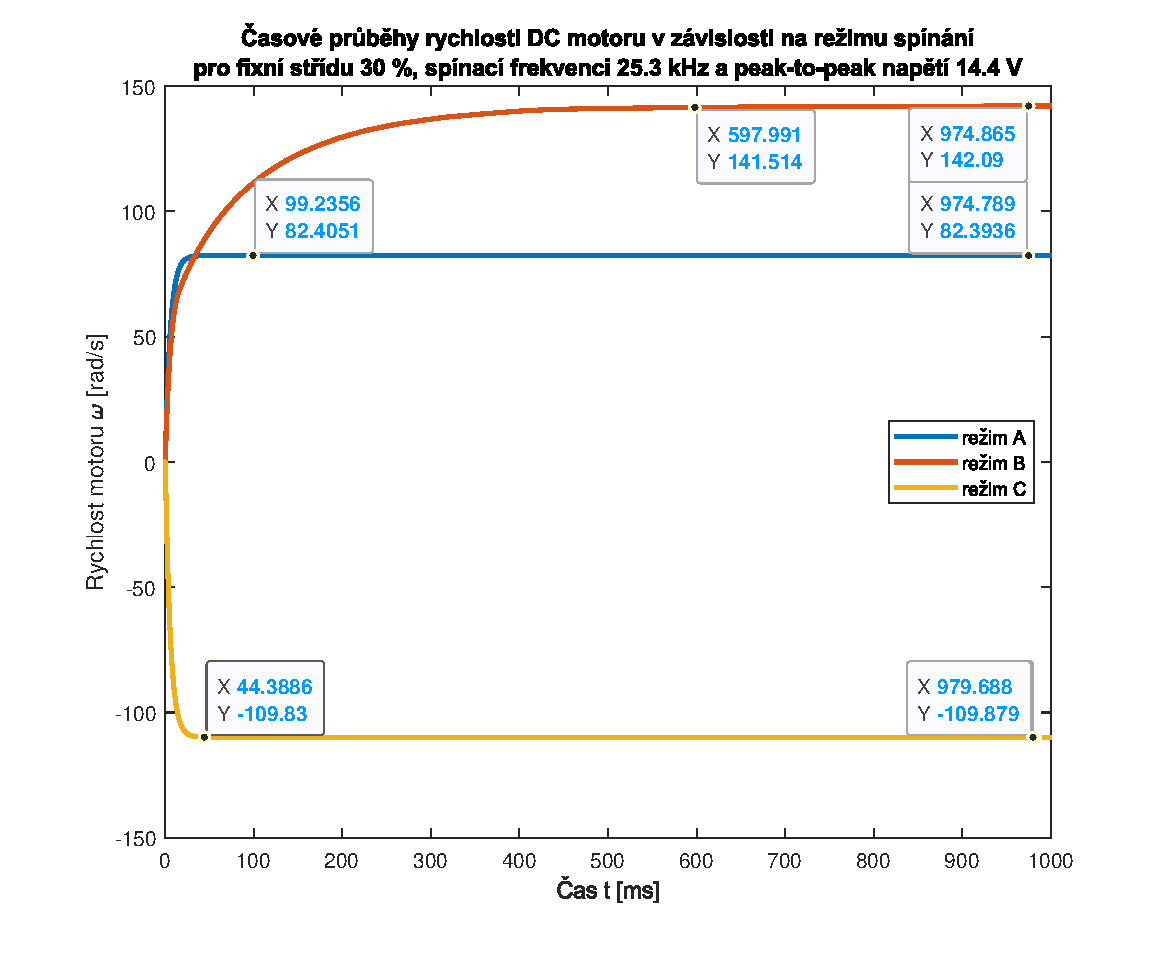
\includegraphics[width=\linewidth]{rychlosti.eps}
	\caption{Výstup simulace motoru s H-můstkem}
	\label{fig:rychlosti}
\end{figure}



\end{document}


